\documentclass{article}

\usepackage{geometry}
\usepackage{amsmath}
\usepackage{graphicx}
\usepackage{listings}
\usepackage{hyperref}
\usepackage{multicol}
\usepackage{fancyhdr}
\pagestyle{fancy}
\hypersetup{ colorlinks=true, linkcolor=black, filecolor=magenta, urlcolor=cyan}
\geometry{ a4paper, total={170mm,257mm}, top=20mm, right=20mm, bottom=20mm, left=20mm}
\setlength{\parindent}{0pt}
\setlength{\parskip}{1em}
\renewcommand{\headrulewidth}{0pt}
\lhead{Competitive Programming - Arkavidia V}
\fancyfoot[CE,CO]{\thepage}
\lstset{
    basicstyle=\ttfamily\small,
    columns=fixed,
    extendedchars=true,
    breaklines=true,
    tabsize=2,
    prebreak=\raisebox{0ex}[0ex][0ex]{\ensuremath{\hookleftarrow}},
    frame=none,
    showtabs=false,
    showspaces=false,
    showstringspaces=false,
    prebreak={},
    keywordstyle=\color[rgb]{0.627,0.126,0.941},
    commentstyle=\color[rgb]{0.133,0.545,0.133},
    stringstyle=\color[rgb]{01,0,0},
    captionpos=t,
    escapeinside={(\%}{\%)}
}

\begin{document}

\begin{center}
    \section*{B. Nonogram} % ganti judul soal

    \begin{tabular}{ | c c | }
        \hline
        Batas Waktu  & 1s \\    % jangan lupa ganti time limit
        Batas Memori & 512MB \\  % jangan lupa ganti memory limit
        \hline
    \end{tabular}
\end{center}

\subsection*{Deskripsi}

\textit{Nonogram} atau \textit{Picross} adalah sebuah \textit{game} logika yang dimainkan pada sebuah kisi/tabel kotak-kotak.
Pada sisi atas dan kiri \textit{Nonogram} terdapat sejumlah deretan angka.
Deretan angka tersebut menunjukkan jumlah sel bersebelahan yang terisi pada baris/kolom tersebut.
Deretan sel terisi pada suatu baris tidak dapat menempel dengan deretan sel terisi lainnya
Berikut contoh dari sebuah teka-teki \textit{Nonogram}.

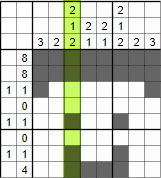
\includegraphics[width=100px]{Homogram-Steve}

Nana sedang menyelesaikan sebuah teka-teki \textit{Nonogram}. 
Nana sudah berhasil mengisi beberapa kolom pada \textit{Nonogram}, dan ia membutuhkan bantuan Anda untuk membantu menyelesaikannya.

Pada soal ini, Anda diberikan sebuah kisi 1xN dari sebuah teka-teki \textit{Nonogram} yang sudah separuh terisi.
Tugas Anda adalah untuk menentukan jumlah konfigurasi yang dapat dibuat agar sesuai dengan nilai di samping kisi dan sel yang sudah terisi.

\subsection*{Format Masukan}

Baris pertama terdiri dari N ($1 \leq N \leq 100.000$), yaitu panjang baris teka-teki \textit{Nonogram}.
$N$ baris berikutnya berisi nilai 0/1, dengan nilai 0 mengindikasikan sel yang masih kosong dan 1 mengindikasikan sel yang sudah terisi.
Baris berikutnya berisi nilai k, yaitu banyaknya angka yang terdapat pada samping kisi teka-teki \textit{Nonogram}.
$k$ baris berikutnya berisi bilangan bulat yang menunjukkan banyak sel yang terisi pada satu deretan.

Contoh:
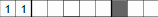
\includegraphics[width=100px]{Homogram-Row}

Pada gambar tersebut, $N$ bernilai 8 dengan deretan nilai [0, 0, 0, 0, 0, 1, 0, 0], dan $k$ bernilai 2 dengan nilai [1, 1].

\subsection*{Format Keluaran}

Keluarkan jumlah kombinasi yang mungkin dibuat dengan syarat pada masukan diatas

Untuk tiap kasus uji, tuliskan $N$ baris, dengan baris ke-$i$ menyatakn jumlah $A_i + B_i + C_i$.
\\

\begin{multicols}{2}
\subsection*{Contoh Masukan}
\begin{lstlisting}
8
0 0 0 0 0 1 0 0
2
1 1
\end{lstlisting}
\columnbreak
\subsection*{Contoh Keluaran}
\begin{lstlisting}
5
\end{lstlisting}
\vfill
\null
\end{multicols}

\pagebreak

\end{document}
